\documentclass{article}
\usepackage[utf8]{inputenc}
\usepackage[margin=1.25in]{geometry}
\usepackage{amsmath}
\usepackage{ amssymb }
\usepackage{ dsfont }
\usepackage{setspace}
\usepackage{graphicx}
\usepackage{physics}
\usepackage{subcaption}
\graphicspath{ {pix/} }

\title{Computational Physics 4}
\author{Jack Donahue}
\begin{document}


\maketitle
%\doublespacing

\begin{abstract}
In this report we investigate the time integration of the ordinary differential equations of orbital mechanics. We begin by studying a variety of different methods used to solve for the orbit of mars, with attention given to the rates of convergence and conservation of energy throughout the orbit. We then write an adaptive time step method for the orbit of Halley's Comet, which has a significantly longer period than that of Mars. We investigate which has the shortest run-time to achieve a given accuracy. Finally, we add in general relativistic effects by  changing the normal Newtonian potential to compute the procession of the star S2, which will be measured experimentally in the coming years
\end{abstract}
\section*{Introduction}
Many interesting physical problems require evolving a system from one time to another. In previous reports, we dealt with pressure and density fields but here we deal with a simpler point particle. Solving the equations of motions usually involves solving some ordinary differential equations. While this may seem like a simple problem, there are a wealth of different ways to solve it. As we will see, different time integration techniques will have trade-offs and convergence rates  in the next section.

The orbits of heavenly bodies has long interested humans who've turned their eyes to the sky. Many of the solutions were found in a time before the steam engine, let alone the computer. Therefore, it presents a nice historical testing grounds for our investigation of these different methods. In the case of S2, a star which orbits the black hole at the center of our universe, we have yet to measure the procession that we will calculate in this report. So despite the simplicity of the problem, it's also a useful physical situation to study and understand. The Newtonian potential is given by $\phi_N = -GM/r$ where G is the gravitational constant and M the mass of the attracting object. This leads to equations of motion of the form
\begin{equation}
  \frac{d^2x}{dt^2}=-\frac{GM x}{r^3} \,\,\,\, \mbox{and} \,\,\,\, \frac{d^2y}{dt^2}  = - \frac{GM y }{r^3}.
\end{equation}
These two ordinary differential equations (ODE) can be made into four first order ODE's by the definition $v=\frac{dx}{dt}$. With this, we can apply the methods of the next system to our four element state vector $r = (x,y,v_x,v_y)$.

\section*{Method}
In this report we will use a variety of different methods for both root-finding and time integration methods. In this section we will briefly review the form of each and their theoretical advantages and convergence rates. 

\subsection*{Forward-Euler}
Forward Euler is one of the simplest methods to solve ODEs. It is given by
\begin{equation}
    f(x+h) = f(x) + h f'(x).
\end{equation}
This method is very clearly first-order and is perhaps only advantageous for it's simplicity in understanding how it works. 

\subsection*{Runge-Kutta}
These methods use trial steps in the middle of the range of integration to cancel lower order terms. We will use two methods RK2 and RK4, which are 2nd-order and 4th-order respectively. RK2 is given by 
\begin{equation}
\begin{split}
    k_1 & = h  f(t,x_n) \\
    k_2 & = h  f(t+\frac{1}{2}h,x+\frac{1}{2}k_1) \\
    x_{n+1} & = x_n + k_2 + O(h^3)
\end{split}
\end{equation}
and RK4 by
\begin{equation}
\begin{split}
    k_1 & = h f(t,x_n)                                \\
    k_2 & = h f(t+\frac{1}{2}h,x+\frac{1}{2}k_1)      \\
    k_3 & = h f(t+\frac{1}{2},x+\frac{1}{2}k_2)        \\
    k_4 & = h f(t+h,x+k_3)                             \\
    x_{n+1} & = x_n + \frac{1}{6}(k_1+2 k_2 +2 k_3 + k_4) + O(h^5).
\end{split}
\end{equation}
These methods, especially RK4, are hugely popular for their simplicity to code and accurate and quick evaluations. As we will do later in the report, it is often paired with an adaptive step-size routine.

\subsection*{Verlet}
This method is based on leap-frog methods. These methods are time symmetric and so fundamentally are good at conserving energy in physical systems. This method needs two initial data, $x_n$ and $v)n$, and is given by
\begin{equation}
\begin{split}
v_{n+1/2} & = v_n + \frac{1}{2}f(t,x_n) \\
x_{n+1} & = x_n +h v_{n+1/2} \\ 
k & = h f(t+h, x_{n+1}) \\ 
v_n & = v_{n+1/2} + \frac{1}{2}k  \\
v_{n+3/2} & = v_{n+1/2} +k 
\end{split}
\end{equation}
We can see that after the two initial data points it continues on its own. In fact, this method also calculates the velocities at half time steps. If we were so inclined, we could store these and use them to reconstruct the rest of the orbits, increasing the accuracy of the simulation. We leave that, however, to future projects. 

\subsection*{Adaptive Step-Size}
We will use adaptive step-size to extend our RK4 method. Adaptive methods decrease step-size when the change in the function is great, but increase it and speed through boring sections that don't change much. To find out whether or not we can change the step-size, we need to compute RK4 twice with half the step size and once with a full step. If the difference between these two is small, then we accept the step and increase the step size. If it is too large, where large is set by the algorithm we use, then the evaluations are discarded the step size decreased and we try again. This seems like a disadvantage, we evaluate RK4 three times instead of just once. The gain, however, is increased accuracy when we need it and speed when things are boring. Overall, adaptive step-sizes usually reduce the run-time and accuracy of a program. 

\subsection*{Newton-Raphson}
We now move in to root finding techniques. This technique converges quadratically for most functions that we'll care about. It is given by
\begin{equation}
    x_{n+1} = x_n - \frac{f(x_n)}{f'(x_n)}.
\end{equation}
A possible disadvantage of this method is that one must know the derivative of the function one wishes to find the root of. 

\subsection*{Bisection}
This method is quite simple and doesn't have a simple equation form. The algorithm works by repeatedly bracketing the root until we're close enough to call it a day. One starts with two points in the domain that evaluate to positive and negative. If there's only one root, we know it must be between them. We choose the midpoint and evaluate it, then use it to replace the other point with the same sign as it has. This method works by slowly walking towards the root. It converges linearly.

\subsection*{Relaxation}
The relaxation method i another simple method. It consists of repeated guesses of the function we want to minimize, given by
\begin{equation}
    x_{n+1} = x_n - f(x_n).
\end{equation}
This method will diverge in general so we must have $|f'(x) < 1|$ in our testing region. 

\subsection*{Secant}
This final method is similar to Newton-Raphson, with the advantage that we do not need to know the derivative in order to use it. This makes it easier to generalize to higher-dimenions and more complicated funcitons. It is given by
\begin{equation}
    x_{n+1} =x_n - f(x_n)\frac{x_n-x_{n-1}}{f(x_n)-f(x_{n-1})}.
\end{equation}
The convergence rate is the golden ration, about 1.6, worse than Newton-Raphson's quadratic convergence. 

\subsection*{Orbits}
We will investigate three different problems of orbital mechanics. The first will be calculating the orbit of Mars for 5 earth years. This case is well-behaved and an easy ellipse so we will use it to compare different algorithms. We will compute the exact method of the orbit by finding the root of the solution to the eccentric anomaly, given by $f(x) = x - e*sin(x) - T \sqrt{a^{-3}}$ where e is the eccentricity, a the semi-major axis, T is the time we care about, and x the angle made with respect to the semi-major axis. The error of the different methods will be computed with respect to the solution of the above equation, found by Newton-Raphson with a large number of iterations. We will then compare the convergence we found with respect to the theoretically predicted value. We will also compare the convergence rates of other root-finding methods to the solution found with a large number of Newton-Raphson iterations. 

We will then move on to the problem of Halley's comet. This comet has a long period of orbit, about 75 years. During a long time, it is moving quite slowly so is a choice problem to which we can apply adaptive RK4. We will compare this solution and run-time with non-adaptive RK4 and Verlet. 

Finally, we will investigate the star S2 wich orbits the black hole in the center of the Milky Way. It is close enough that the effects of general relativity affects the orbit. To take this into account, we modify the Newtonian potential, $\phi_N$, to the Paczynski-Wiita potential $\phi_{PW} = -GM/(r-r_s)$ where $r_s = 2GM/c^2$ is the Schwarzschild radius. We then compare the difference of the solutions with $\phi_N$ and $\phi_PW$. 

\section*{Results}

An example calculated orbit of Mars in presented in Fig \ref{fig:marsex}, calculated for 5 Julian years at 1000 steps. The methods used and shown are Forward Euler, RK2, RK4 and Verlet. The energy time graph is displayed on top while the track of each method is shown below. The convergence rates for the different methods are shown in Figure \ref{fig:marsconv}. We find that at large N, all but Euler have a convergence rates of 1. We find that Euler is again the worst, but at some high step number drops quickly. 

Fig \ref{fig:rootconv} shows the convergence of the Secant, Bisection and Relaxation method root finders. The secant method was found to converge the fastest at 2.66 while the bisection mehtod converged the slowest at 0.3. 

An example of an orbit of Halley's comet is found in Figure \ref{fig:halley}, with 3 periods of orbit and 6000 steps. The methods used and shown are non-adaptive RK4, Verlet and adaptive RK4. The energy is graphed by step, by which we can see that the adaptive method actually finished in fewer steps. We can see that Verlet had a regular period and energy, but began to process. Finally, non-adaptive RK4 began to loose energy very quickly and so its period hastened. 

In Figure \ref{fig:halleyconv} we present the convergence rates of different methods as applied to the problem of two periods of the orbit of Halley's comet. As we can see, the non-adaptive methods do not catch up to the adaptive method up to 50000 time steps. At this point, the adaptive method only takes 7 second to run while the RK4 takes 30 seconds and the Verlet 8 seconds. 

An example procession is shown in Fig \ref{fig:gr}. At one point the code created this beauty, but then it broke and could not be recovered in time. 


\section*{Discussion}

The methods for the simulation of the orbit of Mars all seem to converge at a rate of 1, except for Forward-Euler. This is welcomed and expected for RK2 and Verlet, but not for RK4. I could not find why it converged slower than expected. We note, however, that theoretical scaling is just that, theoretical. And was matters is the specific problem and parameters the method is applied to. We find that it takes about 300 steps total, or about 100 per orbit, before the theoretical scaling laws begin. This is no doubt a function of the curvature of the orbit. At about 100 steps, we resolve the orbit well enough for convergence onto the exact orbit to begin. 

For the methods RK2 RK4 and Verlet the code seems to conserve energy really well over the 5 years simulated. We expect, however, that over long times only the Verlet method will conserve energy well. Forward Euler is just terrible overall, running wild quite quickly. Interesting, Verlet seems to get things wrong in the first step but then remains constant for the rest of the simulation. 

The root finding methods converge overall as expected. We find that the secant does better than expected, converging in about 3 iterations total. Bisection does worse than expected, converging at a third of the rate we expect.

Haley's comet complicated things quite a bit. The adaptive RK4 has an arbitrarily set accuracy, but one that could not be matched by RK4 or Verlet up to 50000 time steps! At this point, the other methods were running way longer than the adaptive. This makes sense, as we expected the adaptive to go slow where needed. If we made Verlet or RK4 go that slow it would have to do it for the whole orbit and I'd still be sitting here!

To get the procession to show up, we need to constrain the error to be below the order of the correct $r_S$. This means that it takes quite a bit for our code to run and resolve the procession. Sadly the procession was once encountered and is shown in this report but couldn't be coaxed back out of the code, so I don't have the numbers of the procession rate. Hopefully the astronomers looking for this will write better code than I (there's no doubt they will). 

\section*{Conclusion}

We see that even for the 'simple' problem of a set of ordinary differential equations, there are a wealth of different integration methods with different advantages and disadvantages. The adaptive RK4 comes out as the clear winner in my book. It made Haley's comet look like and easy problem and had no trouble implementing GR effects. It would be interesting to see if one could simulate the procession of Mercury, but as that is a smaller effect than the procession of S2 which itself took a long time to run, I'm not so sure it'd be totally worth it. 



\begin{figure}[h]
    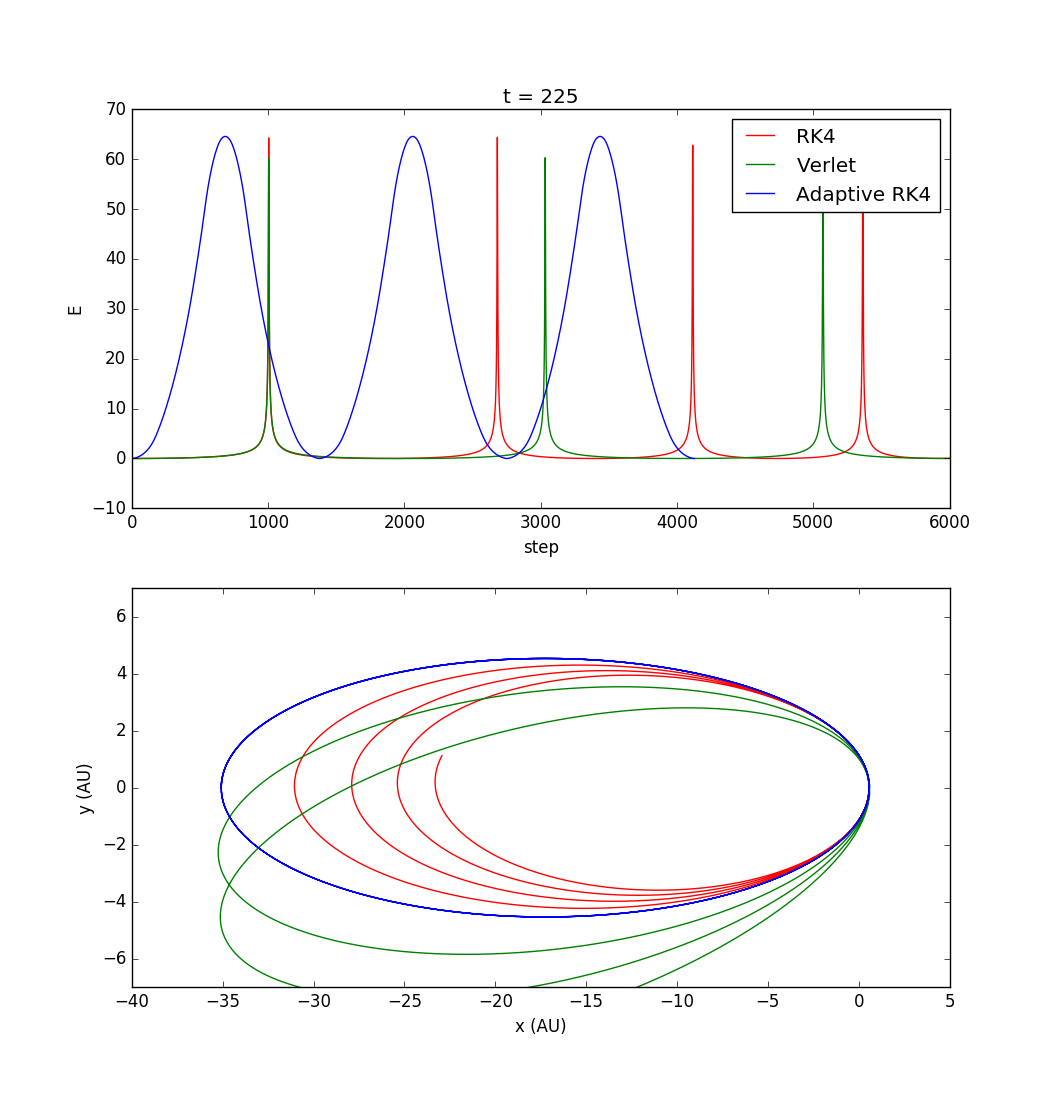
\includegraphics[width=\textwidth]{halley6000_3.png}
    \caption{Simulation of Haley's comet's orbit for three periods, 6000 time steps. On top we display the energy versus time-step for each method, energy with units of $M_\odot\frac{{AU}^2}{yr^2}$. Notice that the adaptive method completes in fewer total steps. The bottom plots shows the track of each method. Notice the procession of the Verlet method and the energy loss of non-adaptive RK4 }
    \label{fig:halley}
\end{figure}

\begin{figure}[h]
    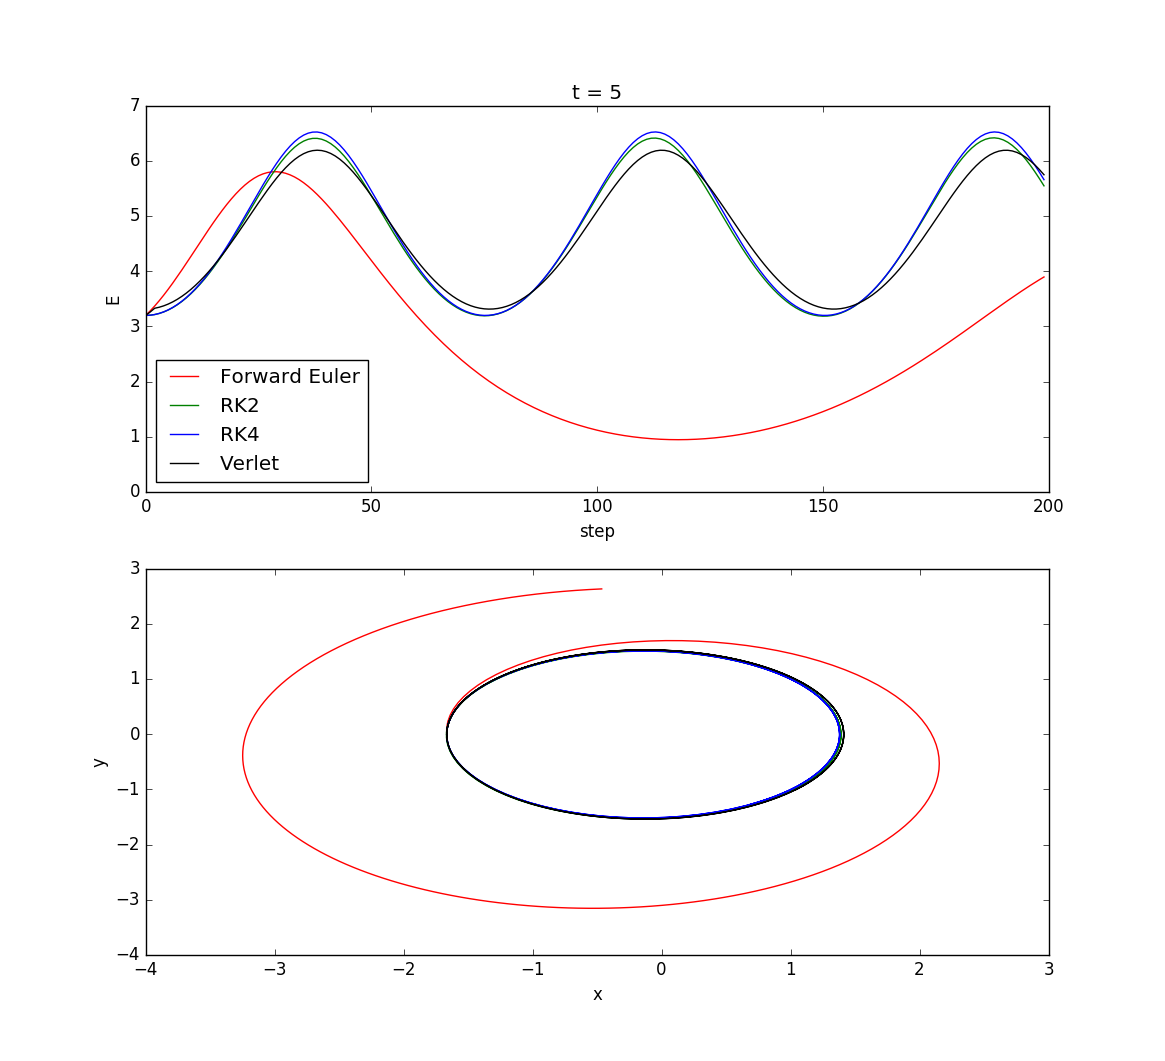
\includegraphics[width=\textwidth]{MarsOrbit.png}
    \caption{Simulation of the orbit of Mars about the Sun for 5 Earth years, about 2.66 periods of Mars. On top is the energy of each orbit with step (=time as steps are constant size). Notice that over the 5 years all but Forward-Euler conserve the energy well. In the plot of the tracks, we see that the Forward Euler method runs wild while the others stay constant.  }
    \label{fig:marsex}
\end{figure}

\begin{figure}[h]
    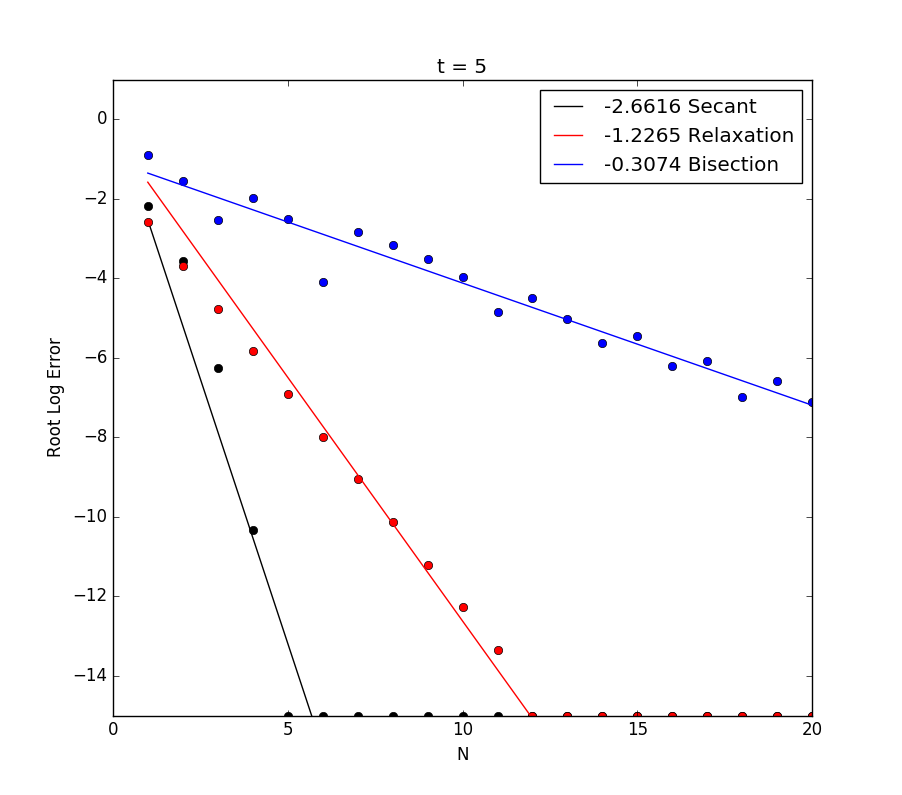
\includegraphics[width=\textwidth]{rootconv.png}
    \caption{The convergence of root finding methods with iteration steps. The error is computed with respect to Newton-Raphson with a large number of steps. The secant method converges the quickest out of the three as expected.}
    \label{fig:rootconv}
\end{figure}

\begin{figure}[h]
    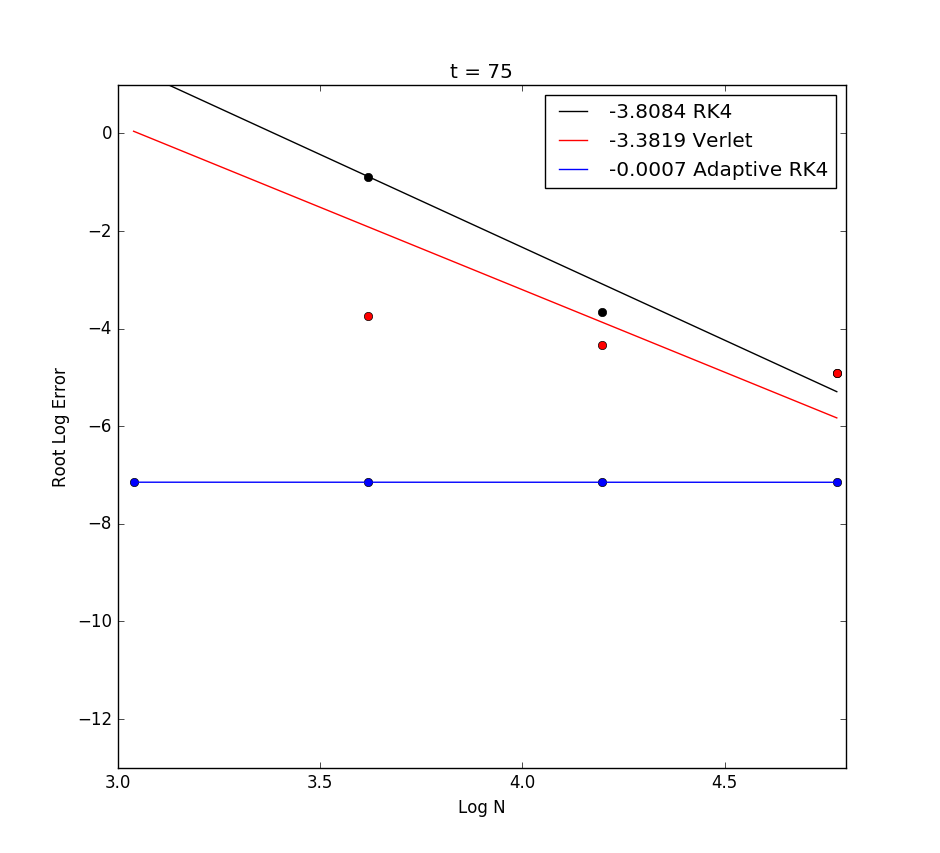
\includegraphics[width=\textwidth]{halleyconv.png}
    \caption{Here we show the convergence of the three different methods for the problem of two periods of Halley's comet. Interesting, up to 50000 time steps, the other methods never become as accurate as the adaptive method. At that stage, the other methods begin to run significantly longer than the adaptive method.}
    \label{fig:halleyconv}
\end{figure}

\begin{figure}[h]
    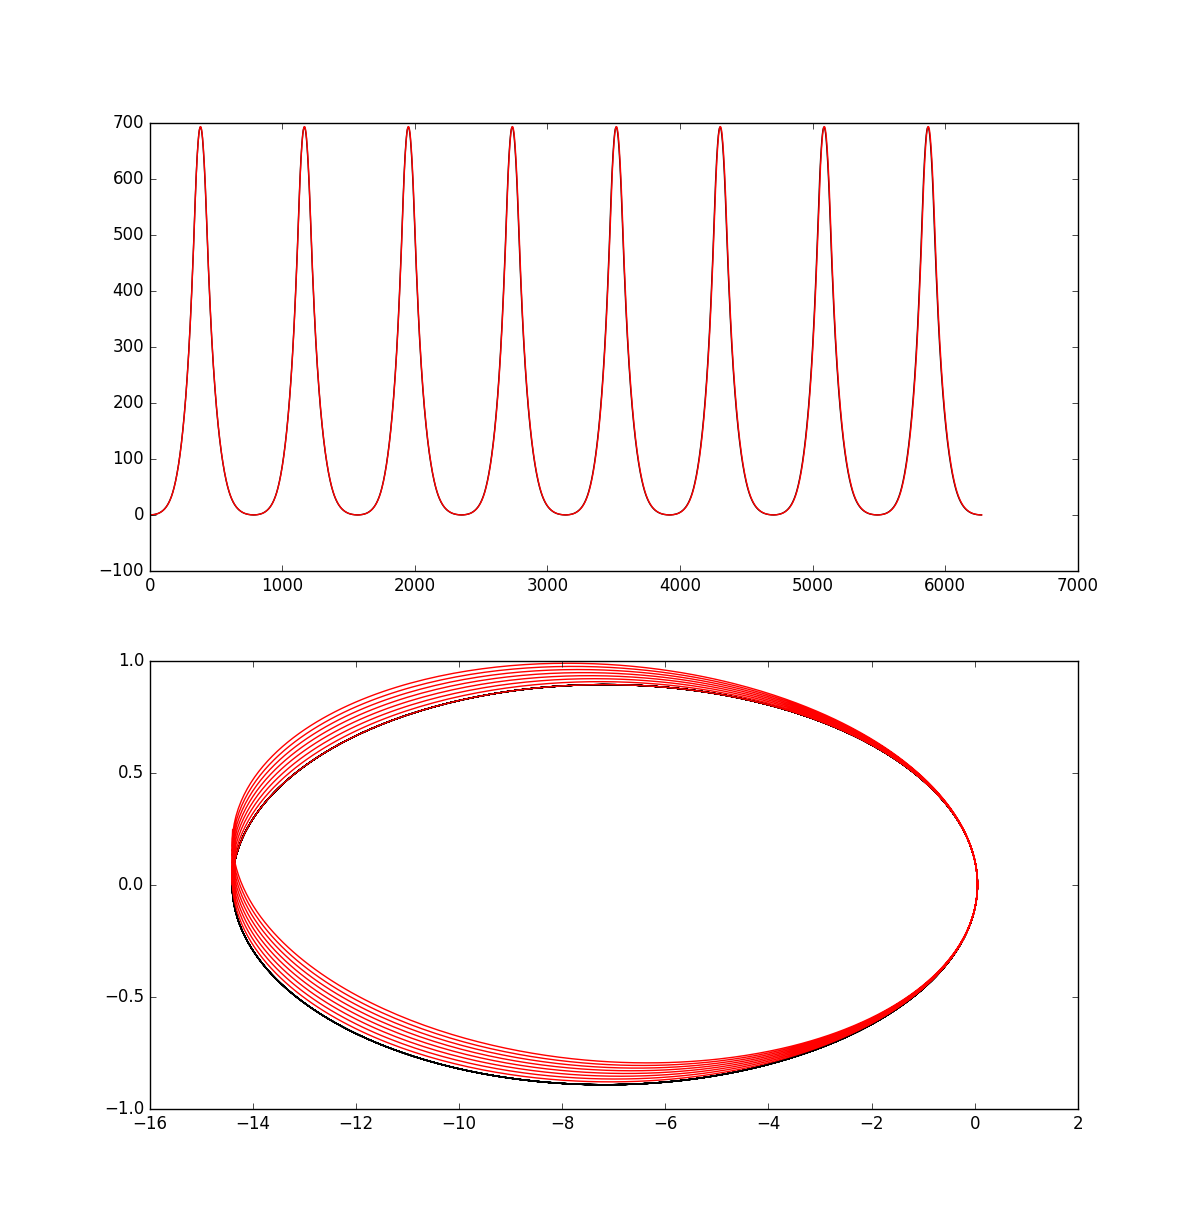
\includegraphics[width=\textwidth]{s2.png}
    \caption{This is one example of the procession found for the GR example. We see that the energy for both schemes with and without GR effects that energy is conserved. Interestingly, the GR effects lead to procession of the orbit.}
    \label{fig:gr}
\end{figure}

\begin{figure}[h]
    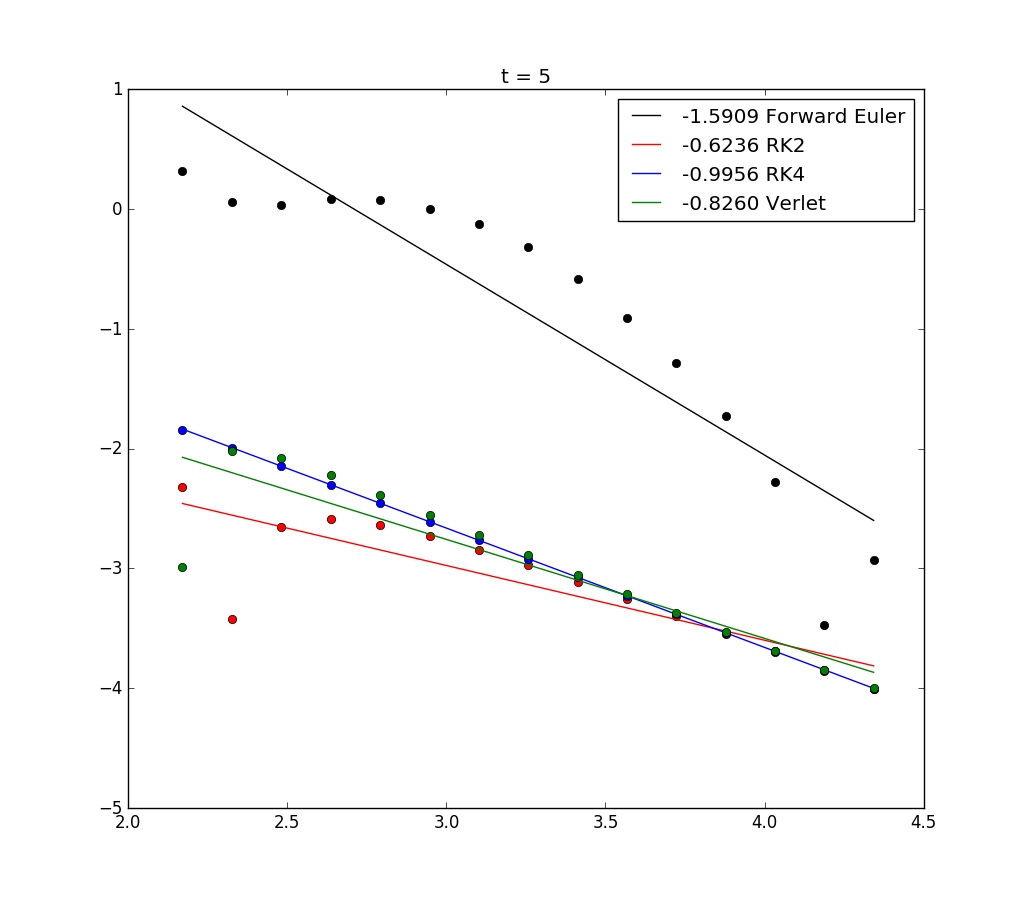
\includegraphics[width=\textwidth]{marsconv.png}
    \caption{Convergence rates and plots for the orbiting of Mars for 5 Earth years. There are about 2.66 Mars years in 5 Earth years so we see that it takes about 100 steps per orbit before theoretical scaling begins.}
    \label{fig:marsconv}
\end{figure}


\end{document}
